\section{Cost Estimating}\label{cost-estimating}

In order to understand how to include cost estimates, it may be helpful to first define some terminology and provide an overview of the process used in EnergyPlus. There are three broad steps involved. The first involves determining \emph{construction} costs by summing individual ``line items.''~ The second involves determining \emph{project} costs by adjusting construction costs to account for things like profit and design fees. The third involves comparing the current simulation to a reference case so that marginal increases can be calculated. Each of these steps involves using one of the three `ComponentCost' objects described below.

\subsection{ComponentCost:LineItem}\label{componentcostlineitem}

Each instance of this object creates a cost line item and will contribute to the total for a cost estimate. Each line item is reported in table form in the tabular report file. The user must request that this report be generated by including a \hyperref[outputtablesummaryreports]{Output:Table:SummaryReports} object with the Component Cost Economics Summary option selected. The style of a tabular report can be controlled using the \hyperref[outputcontroltablestyle]{OutputControl:Table:Style} object.

Cost estimates are not currently general in that they cannot be performed for every type of component that could be included in an EnergyPlus model. Although a ``General'' option is available where all information needed for the cost line item is input by the user, the usefulness of cost modeling within EnergyPlus is expected to be enhanced when quantities are obtained from elsewhere in the input file or computed during a simulation. The cost computations are programmed in selected ways for selected objects. The objects available and the type of cost modeling that may be performed are discussed in detail in the discussion of Reference Object Type field. A particular instance of this object will always have many blank fields. Entering values in too many fields may cause an error because the program may determine how a particular cost is to be calculated based on the presence of non-zero values in particular fields. The input object includes fields that are reserved for future use in expanded cost estimate and investment analyses planned for future versions of EnergyPlus. If you would like to request additional objects or different methods of modeling component costs, feel free to describe your needs and submit a request via email to energyplus-support@gard.com.

\subsubsection{Inputs}\label{inputs}

\paragraph{Field: Name}\label{componentcostlineitem-field-name}

This field is a user-selected name that will appear in the line item description of the cost report. It is not used in the calculation but allows identifying a line item in the subsequent report.

\paragraph{Field: Type}\label{field-type}

This field is not yet used and may be left blank.

\paragraph{Field: Line Item Type}\label{field-line-item-type}

The cost estimate line item calculation will be controlled by the name entered in this field. The requirements for the remaining input, and the cost calculations performed, will vary depending on the object referenced here. Only selected objects can be entered here. The objects available for cost estimating are listed in the following table showing the active fields and options available for each.

% table 37
\begin{longtable}[c]{p{1.4in}p{0.4in}p{0.4in}p{0.5in}p{0.5in}p{0.4in}p{0.4in}p{0.4in}p{0.4in}p{0.5in}}
\caption{Cost Line Item Types (ref Objects) \label{table:cost-line-item-types-ref-objects}} \tabularnewline
\toprule
Object Types available (choice keys) & Cost per each & Cost per m\(^{2}\) & Cost per kW & Cost per kW*COP & Cost per m\(^{3}\) & Cost per m\(^{3}\)/s & Cost per W/K & Qty & Wildcard for Name \tabularnewline
\midrule
\endhead

General & X & ~ & ~ & ~ & ~ & ~ & ~ & X & ~ \tabularnewline
\hline
Construction & ~ & X & ~ & ~ & ~ & ~ & ~ & ~ & ~ \tabularnewline
\hline
Coil:DX Coil:Cooling:DX: SingleSpeed & X & ~ & X & X & ~ & ~ & ~ & ~ & X \tabularnewline
\hline
Coil:Heating:Fuel & X & ~ & X & X & ~ & ~ & ~ & ~ & X \tabularnewline
\hline
Chiller:Electric & X & ~ & X & X & ~ & ~ & ~ & ~ & ~ \tabularnewline
\hline
Daylighting:Controls & X & ~ & ~ & ~ & ~ & ~ & ~ & ~ & X \tabularnewline
\hline
Shading:Zone:Detailed & ~ & X & ~ & ~ & ~ & ~ & ~ & ~ & ~ \tabularnewline
\hline
Lights & X & ~ & X & ~ & ~ & ~ & ~ & ~ & ~ \tabularnewline
\hline
Generator:Photovoltaic & ~ & ~ & X & ~ & ~ & ~ & ~ & ~ & ~ \tabularnewline
\bottomrule
\end{longtable}

\subparagraph{General}\label{general}


This choice of object is used to calculate costs in a general way. No quantities from internal calculations are used. All information needed for the cost line item is input by the user. The Cost per Each and the Quantity fields that follow need to have values.

\subparagraph{Construction}\label{construction-costlineitem}

This choice of object type is used to calculate the costs associated with surfaces based on the type of \hyperref[construction-000]{Construction} used for the surface. Costs are entered on a per-square-meter basis. The program finds all the surfaces that have the type of \hyperref[construction-000]{Construction} named in the Reference Object Name field that follows and determines the total area. If the model includes duplicate surfaces, as for interior partitions or floors, these will be detected and not double-counted. The cost entered in \hyperref[field-cost-per-area]{Cost per Area} field (\$/m\(^{2}\)) is used for each surface. The line item subtotal is calculated by multiplying the number of units by \hyperref[field-cost-per-area]{Cost per Area}. The \hyperref[field-cost-per-area]{Cost per Area} should include all the material layers defined in the \hyperref[construction-000]{Construction}.

\subparagraph{Coil:DX or Coil:Cooling:DX:SingleSpeed}\label{coildx-or-coilcoolingdxsinglespeed}

This choice of object type is used to calculate the cost of direct expansion cooling equipment. Cost can be entered in three different ways, (1) per each, (2) per kW total cooling capacity, or (3) per kW total cooling capacity per COP (coefficient of performance). The program will determine which method to use by examining which input fields have non-zero values. It is an error to specify costs in more than one way. The per-each approach is most useful for discrete packages. The per-kW approach is useful for autosizing DX coils with the same COP. The per-kW-per-COP approach is convenient for modeling autosized DX coils with differing COPs as long as a linear relationship is sufficient.

The wildcard character ``*'' may be used in the object name field that follows to allow a single line item to include all of the DX coils in the model.

\subparagraph{Coil:Heating:Fuel}\label{coilheatinggas}

This choice of object type is used to calculate the cost of gas-fired heating equipment. Cost can be entered in three different ways, (1) per each, (2) per kW of heating capacity, or (3) per kW total cooling capacity per nominal efficiency (actually uses the per kW per COP field). The program will determine which method to use by examining which input fields have non-zero values. It is an error to specify costs in more than one way. The per-each approach is most useful for discrete packages. The per-kW approach is useful for autosizing heating coils with the same efficiency. The per-kW-per-Eff approach is convenient for modeling autosized heating coils with differing efficiencies as long as a linear relationship is sufficient.

The wildcard character ``*'' may be used in the object name field that follows to allow a single line item to include all of the gas heating coils in the model.

\subparagraph{Chiller:Electric}\label{chiller-electric-costlineitem}

This choice of object type is used to calculate the cost of a central chiller. The object name entered in following field must correspond to a \hyperref[chillerelectric]{Chiller:Electric} object name defined elsewhere in the input file. Cost can be entered in three different ways, (1) per each, (2) per kW total cooling capacity or (3) per kW total cooling capacity per COP (coefficient of performance). The program will determine which method to use by examining which input fields have non-zero values. It is an error to specify costs in more than one way. The per-each approach is most useful for discrete chillers. The per-kW approach is useful for autosizing chillers with the same COP. The per-kW-per-COP approach is convenient for modeling autosized chillers with differing COPs as long as a linear relationship is sufficient.
\subparagraph{Daylighting:Controls}\label{daylightingcontrols}

These choices of object type are used to include the cost of controllers needed to control electric lighting in response to daylight. The only option for entering costs is ``per each''. The wildcard character ``*'' may be used in the following object name field to allow a single line item to include all of the simple and detailed daylighting controls in the cost model.

\subparagraph{Shading:Zone:Detailed}\label{shadingzonedetailed}

This choice of object type is used to calculate the costs associated with attached shading surfaces. Costs are entered on a per-square-meter basis. The cost calculations are similar to those for heat transfer surfaces but are handled separately because ``Construction'' is not defined for a shading surface. The object name entered in the following field must correspond to a \hyperref[shadingzonedetailed-000]{Shading:Zone:Detailed} object name defined elsewhere in the input file.

\subparagraph{Lights}\label{lights}

This choice of object is used to calculate the costs associated with electric lighting. Costs are entered on either a cost-per-each basis or as a cost-per-kilowatt-of-design-level. (This design level is an input in the \hyperref[lights-000]{Lights} object.). The object name entered into the following field must match the name of a Zone object defined elsewhere in the input file.

\subparagraph{Generator:Photovoltaic}\label{generatorphotovoltaic}

This choice of object is used to calculate the costs associated with a photovoltaic system. Costs are entered on a cost-per-kilowatt-of-rated-capacity. The rated capacity of a photovoltaic generator is calculated for cost modeling by exposing the surface to a 1000 W/m\(^{2}\) incident radiation using the area fraction and nominal fixed efficiency input by the user (from the \hyperref[generatorphotovoltaic-000]{Generator:Photovoltaic} object). The object name entered into the following field must match the name of a \hyperref[generatorphotovoltaic-000]{Generator:Photovoltaic} ~object defined elsewhere in the input file.

\paragraph{Field: Item Name}\label{field-item-name}

This field is used to refer to a specific instance of an object. The wildcard character ``*'' is acceptable for some objects as described above for the previous field.

\paragraph{Field: Object End Use Key}\label{field-object-end-use-key}

This field is not yet used and may be left blank.

\paragraph{Field: Cost per Each}\label{field-cost-per-each}

This field is used to enter cost information on a per-each basis. The units are dollars (\$).

\paragraph{Field: Cost per Area}\label{field-cost-per-area}

This field is used to enter cost information on a per-area basis. The units are dollars per square meter (\$/m\(^{2}\)).

\paragraph{Field: Cost per Unit of Output Capacity}\label{field-cost-per-unit-of-output-capacity}

This field is used to enter cost information on a per-kilowatt basis. The units are dollars per kilowatt (\$/kW).

\paragraph{Field: Cost per Unit of Output Capacity per COP}\label{field-cost-per-unit-of-output-capacity-per-cop}

This field is used to enter cost information on a per-kilowatt-per-COP basis. The units are dollars per kilowatt per non-dimensional COP (\$/kW-COP).~ Note that this field can be used for \hyperref[coilheatinggas-000]{Coil:Heating:Fuel} cost modeling in which case the better terminology would be per-kilowatt-per-non-dimensional-efficiency.

\paragraph{Field: Cost per Volume}\label{field-cost-per-volume}

This field is not yet used but will be used to enter cost information on a per-cubic-meter basis. The units are dollars per cubic meter (\$/m\(^{3}\)).

\paragraph{Field: Cost per Volume Rate}\label{field-cost-per-volume-rate}

This field is not yet used but will be used to enter cost information on a per-cubic-meter-per-second basis. The units are dollars per cubic meter (\$/(m\(^{3}\)/s)).

\paragraph{Field: Cost per Energy per Temperature Difference}\label{field-cost-per-energy-per-temperature-difference}

This field is not yet used but will be used to enter cost information on a per-watt-per-Kelvin basis. These units will be used to represent a UA description of coils and the like. The units are dollars per watt per delta K (\$/(W/K)).

\paragraph{Field: Quantity}\label{field-quantity}

This field is used to directly enter the line item quantity. The units should correspond to what is used in the Per Each field.

Some examples of this object in an IDF:

\begin{lstlisting}

  ComponentCost:LineItem,
     PSZ Equipment from scaling , !- Name
     ,                            !- Type
     Coil:DX,                     !- Line Item Type
     ACDXCoil ZN1 ,               !- Item Name
     ,                            !- Object End Use Key
     ,                            !- Cost per Each {$}
     ,                            !- Cost per Area {$/m2}
     ,                            !- Cost per Unit of Output Capacity {$/kW}
     82.5;                   !- Cost per Unit of Output Capacity per COP {$/kW}


    ComponentCost:LineItem,
      Lighting Equip: ZN2_E_Space_1, ,
      Lights,!- Line Item Type
      ZN2_E_Space_1, ,
      ,!- Cost per Each {$}
      ,!- Cost per Area {$/m2}
      3300.000;!- Cost per Unit of Output Capacity {$/kW}




    ComponentCost:LineItem, DL controls: ZN4_W_Space_1, ,
      Daylighting:Detailed, !- Line Item Type
      ZN4_W_Space_1, ,!- Item Name
      125.000, !- Cost per Each {$}
      ,!- Cost per Area {$/m2}
      ;!- Cost per Unit of Output Capacity {$/kW}
\end{lstlisting}

\subsection{ComponentCost:Adjustments}\label{componentcostadjustments}

This object can be used to perform various modifications to the construction costs to arrive at an estimate for total project costs. This object allows extending the line item model so that the overall costs of the project will reflect various profit and fees. Only one object of this type can be included in the input file. The results are included in the Construction Cost Estimate Summary table by request using the \hyperref[outputtablesummaryreports]{Output:Table:SummaryReports} object with the Component Cost Economics Summary option selected.

\subsubsection{Inputs}\label{inputs-1}

\paragraph{Field: Miscellaneous Cost per Conditioned Area}\label{field-miscellaneous-cost-per-conditioned-area}

This optional field can be used to enter a cost model for miscellaneous project costs that are not included in the line item modeling. Miscellaneous costs are entered in dollars per square meter of conditioned floor area. This field allows including the costs of project elements that go beyond what can be modeled using ``\hyperref[componentcostlineitem]{ComponentCost:LineItem}'' input objects including such things as structural components, site preparation, finishes, etc. The value input in this field will be multiplied by the conditioned floor area and listed in the Construction Cost Estimate Summary table. The miscellaneous project costs are added to the line item model total to determine the ``modeled and miscellaneous Construction costs'' that will be multiplied by the fractions in the following five fields.

\paragraph{Field: Design and Engineering Fees}\label{field-design-and-engineering-fees}

This optional field can be used to enter a fraction of modeled and miscellaneous construction costs that should be added to account for design and engineering fees. Note that is not the same as a fraction of the total cost estimate.

\paragraph{Field: Contractor Fee}\label{field-contractor-fee}

This optional field can be used to enter a fraction of modeled and miscellaneous construction costs that should be added to account for Contractor fees. Note that is not the same as a fraction of the total cost estimate.

\paragraph{Field: Contingency}\label{field-contingency}

This optional field can be used to enter a fraction of modeled and miscellaneous construction costs that should be added for contingency. Note that is not the same as a fraction of the total cost estimate.

\paragraph{Field: Permits, Bonding and Insurance}\label{field-permits-bonding-and-insurance}

This optional field can be used to enter a fraction of modeled and miscellaneous construction costs that should be added to account for permitting, bonding, and insurance costs to the project. Note that is not the same as a fraction of the total cost estimate.

\paragraph{Field: Commissioning Fee}\label{field-commissioning-fee}

This optional field can be used to enter a fraction of modeled and miscellaneous construction costs that should be added to account for commissioning services. Note that is not the same as a fraction of the total cost estimate.

\paragraph{Field: Regional Adjustment Factor}\label{field-regional-adjustment-factor}

This optional field can be used to enter an adjustment factor to account for regional differences is construction costs. The factor will be applied to the modeled and miscellaneous construction costs to determine and amount that should be added, or subtracted, to account for local variations in construction costs. The default factor is 1.0. The additive adjustment is calculated by subtracting 1.0 from the value entered in this field. This field is useful for using national average data in the line item and miscellaneous construction cost models and then altering the results based on regional differences.

An example of this object in an IDF is:

\begin{lstlisting}
ComponentCost:Adjustments,
            467, !- Miscellaneous Cost per Conditioned Area
           0.07, !- Design and Engineering Fees
           0.07, !- Contractor Fee
           0.10, !- Contingency
           0.04, !- Permits, Bonding and Insurance
           0.015,!- Commissioning Fee
          1.136; !- Regional Adjustment Factor
\end{lstlisting}

\subsection{ComponentCost:Reference}\label{componentcostreference}

This object can be used to allow comparing the current cost estimate to the results of a previous estimate for a reference building. This object parallels the ComponentCost:Adjustment object but adds a field for entering the cost line item model result for the reference building. All the various adjustments to the project cost estimate are available here to allow using factors that differ between the current and the reference building models. The factors entered in the field associated with this object are applied to the reference building while the factors listed in the ComponentCost:Adjustment object are applied to the current building model cost estimate. Only one object of this type can be included in the input file. The results are included in the Construction Cost Estimate Summary table by request using the \hyperref[outputtablesummaryreports]{Output:Table:SummaryReports} object with the Component Cost Economics Summary option selected.

\subsubsection{Inputs}\label{inputs-2}

\paragraph{Field: Reference Building Line Item Costs}\label{field-reference-building-line-item-costs}

This field is used to enter a dollar amount representing the total for the reference building that the user would like to compare to the line item cost model for the current building model. A typical source of data for this would be the ``Line Item Subtotal'' from a previous EnergyPlus simulation.

\paragraph{Field: Reference Building Miscellaneous Cost per Conditioned Area}\label{field-reference-building-miscellaneous-cost-per-conditioned-area}

This optional field can be used to enter a cost model for miscellaneous project costs that are not included in the line item modeling. Miscellaneous costs are entered in dollars per square meter of conditioned floor area. This field allows including the costs of project elements that go beyond what can be modeled using ``\hyperref[componentcostlineitem]{ComponentCost:LineItem}'' input objects including such things as structural components, site preparation, finishes, etc. The value input in this field will be multiplied by the conditioned floor area and listed in the Construction Cost Estimate Summary table. The miscellaneous project costs are added to the reference building line item subtotal to determine the ``modeled and miscellaneous construction costs'' that will be multiplied by the fractions in the following five fields.

\paragraph{Field: Reference Building Design and Engineering Fees}\label{field-reference-building-design-and-engineering-fees}

This optional field can be used to enter a fraction of modeled and miscellaneous construction costs that should be added to account for design and engineering fees. Note that is not the same as a fraction of the total cost estimate.

\paragraph{Field: Reference Building Contractor Fee}\label{field-reference-building-contractor-fee}

This optional field can be used to enter a fraction of modeled and miscellaneous construction costs that should be added to account for Contractor fees. Note that is not the same as a fraction of the total cost estimate.

\paragraph{Field: Reference Building Contingency}\label{field-reference-building-contingency}

This optional field can be used to enter a fraction of modeled and miscellaneous construction costs that should be added for contingency. Note that is not the same as a fraction of the total cost estimate.

\paragraph{Field: Reference Building Permits, Bonding and Insurance}\label{field-reference-building-permits-bonding-and-insurance}

This optional field can be used to enter a fraction of modeled and miscellaneous construction costs that should be added to account for permitting, bonding, and insurance costs to the project. Note that is not the same as a fraction of the total cost estimate.

\paragraph{Field: Reference Building Commissioning Fee}\label{field-reference-building-commissioning-fee}

This optional field can be used to enter a fraction of modeled and miscellaneous construction costs that should be added to account for commissioning services. Note that is not the same as a fraction of the total cost estimate.

\paragraph{Field: Reference Building Regional Adjustment Factor}\label{field-reference-building-regional-adjustment-factor}

This optional field can be used to enter an adjustment factor to account for regional differences is construction costs. The factor will be applied to the modeled and miscellaneous construction costs to determine and amount that should be added, or subtracted, to account for local variations in construction costs. The default factor is 1.0. The additive adjustment is calculated by subtracting 1.0 from the value entered in this field. This field is useful for using national average data in the line item and miscellaneous construction cost models and then altering the results based on regional differences.

An example of this object in an IDF is:

\begin{lstlisting}

ComponentCost:Reference,
    683060.000, !- Reference Building Line Item Costs {$}
    467.0, !- Reference Building Miscellaneous Cost per Conditioned Area {$/m2}
    0.060, !- Reference Building Design and Engineering Fees {dimensionless}
    0.070, !- Reference Building Contractor Fee {dimensionless}
    0.100, !- Reference Building Contingency
    0.04,  !- Reference Building Permits, Bonding and Insurance {dimensionless}
    0.0075,!- Reference Building Commissioning Fee {dimensionless}
    1.136; !- Reference Building Regional Adjustment Factor {dimensionless}
\end{lstlisting}

\subsection{Economics Cost Estimate Reporting}\label{economics-cost-estimate-reporting}

Cost estimate results are only output to tabular reports; they are not available in the standard output file (.eso). The results are included in the Construction Cost Estimate Summary table by request using the object \hyperref[outputtablesummaryreports]{Output:Table:SummaryReports} object with the Component Cost Economics Summary option selected. The figure below shows an example of summary output using html style for tabular reporting. A second table is produced that provides the line item details with one line for every line item object. Per-area cost modeling and cost normalization are based on total conditioned floor area which is also provided in the tabular report.

\begin{figure}[hbtp] % fig 163
\centering
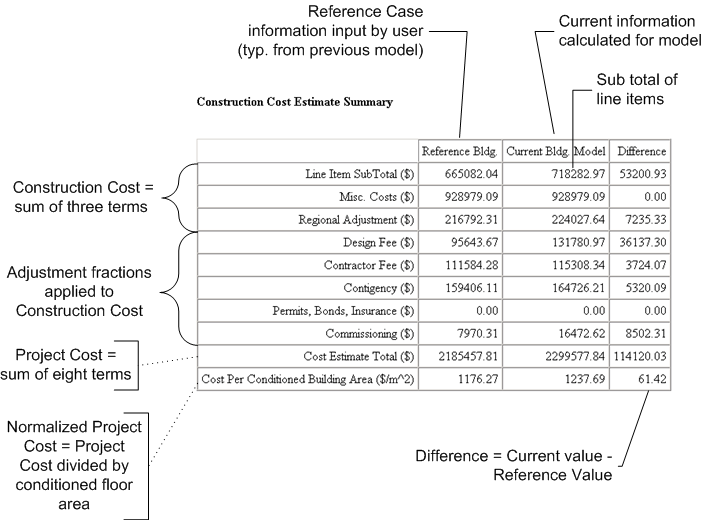
\includegraphics[width=0.9\textwidth, height=0.9\textheight, keepaspectratio=true]{media/image616.png}
\caption{Economics Cost Modeling \protect \label{fig:economics-cost-modeling}}
\end{figure}

``Line Item Subtotal'' is the sum of items explicitly modeled in the cost estimate. For the reference building, this value is input by the user. For the current building, this value is the sum of line items which are detailed in Cost Line Item Details table that follows.

``Misc. Cost'' is the product of the user-defined Miscellaneous Cost Model (per Square Meter) and the conditioned floor area.

``Regional Adjustment'' is the produce of the user-defined Regional Adjustment Factor and the conditioned floor area.

``Design Fee'' is the product of the user-defined Design and Engineering Fee Fraction and the subtotal for construction costs (which includes the Line Item Subtotal, Misc. Cost, and Regional Adjustment).

``Contractor Fee'' is the product of the user-defined Contractor Fee Fraction and the subtotal for construction costs (which includes the Line Item Subtotal, Misc. Cost, and Regional Adjustment).

``Contingency'' is the product of the user-defined Contingency Fraction and the subtotal for construction costs (which includes the Line Item Subtotal, Misc. Cost, and Regional Adjustment).

``Permits, Bonds, and Insurance'' is the product of the Permits, Bonding, Insurance Fraction and the subtotal for construction costs (which includes the Line Item Subtotal, Misc. Cost, and Regional Adjustment).

``Commissioning'' is the product of the user-defined Commissioning Fee Fraction and the subtotal for construction costs (which includes the Line Item Subtotal, Misc. Cost, and Regional Adjustment).

``Cost Estimate Total'' is the sum of eight items above and represents the total project cost estimate.

``Cost per Conditioned Building Area'' is the Cost Estimate Total divided by the total conditioned floor area. This represents a normalized cost intensity.
